\documentclass[11pt]{article}

\usepackage[margin=0.9in]{geometry}
\usepackage{amsmath,amssymb}
\usepackage{array}
\usepackage{booktabs}
\usepackage{graphicx}
\usepackage{microtype}
\usepackage{xcolor}
\usepackage[hidelinks]{hyperref}

\definecolor{resultblue}{RGB}{33,91,147}
\definecolor{caveatred}{RGB}{150,45,45}
\newcommand{\code}[1]{\texttt{#1}}
\newcommand{\Akap}{A_{\kappa}}
\newcommand{\Apre}{A_{\widehat p}}
\newcommand{\Apost}{A_p}
\newcommand{\Rpost}{R_p}
\newcommand{\Mdom}{M}
\newcommand{\Cret}{C}
\newcommand{\RunDiagnostics}[4]{%
  \clearpage
  {\large\bfseries #1: #3}\par
  \vspace{2pt}
  {\footnotesize #4\par}
  \vspace{4pt}
  \begin{center}
  \setlength{\tabcolsep}{2pt}
  \begin{tabular}{@{}cc@{}}
    \textbf{Trained checkpoint} & \textbf{Canonical initialization control} \\
    \multicolumn{2}{c}{\footnotesize Gain distributions} \\
    
\includegraphics[width=0.475\textwidth]{figures/runs/#2/trained_gain_distributions.png} &
    
\includegraphics[width=0.475\textwidth]{figures/runs/#2/init_gain_distributions.png} \\
    \multicolumn{2}{c}{\footnotesize Internal variables versus token position} \\
    
\includegraphics[width=0.475\textwidth]{figures/runs/#2/trained_internals_vs_position.png} &
    
\includegraphics[width=0.475\textwidth]{figures/runs/#2/init_internals_vs_position.png} \\
    \multicolumn{2}{c}{\footnotesize Covariance geometry versus token position} \\
    
\includegraphics[width=0.475\textwidth]{figures/runs/#2/trained_covariance_anisotropy.png} &
    
\includegraphics[width=0.475\textwidth]{figures/runs/#2/init_covariance_anisotropy.png}
  \end{tabular}
  \end{center}
}

\title{Diagonal Kalman Linear Attention:\\
Learned Covariance Anisotropy and Information-Scale Interventions}
\author{Checkpoint diagnostic report}
\date{August 19, 2026}

\begin{document}
\maketitle

\begin{abstract}
We analyze all eleven completed DiagKLA ablation checkpoints with deterministic,
current-code H200 probes.  The primary comparison is a nominally matched 750M family
trained with information scales
$s\in\{1,\sqrt{128},128,512\}$.  A complementary $4\times4$ crossed experiment
holds each trained checkpoint fixed and changes runtime $s$ over the same four values.
The learned gain direction is remarkably stable: nominal trained gain anisotropy stays
near $0.64$ even though canonical initialization controls range from $0.53$ to $0.32$.
Covariance geometry is not scale-invariant.  Nominal posterior anisotropy rises from
$0.641$ to $0.795$, while normalized posterior effective rank falls from $0.721$ to
$0.522$.  In the fixed-weight intervention, changing $s$ from $1$ to $512$ increases
posterior anisotropy in every checkpoint by $0.166$--$0.212$ and reduces posterior
covariance by $87.3\%$--$88.9\%$.  The same intervention rotates the gain only modestly
but strongly reduces its channel-wise magnitude.  DiagKLA therefore learns a robustly
anisotropic gain direction, while \code{info\_scale} primarily controls how strongly
the measurement update contracts and concentrates uncertainty across channels.
These diagnostics establish state geometry, not a causal effect on language-model loss.
\end{abstract}

\tableofcontents

\section{Questions and conclusions}

This report addresses three questions.
\begin{enumerate}
  \item Does trained DiagKLA use channel-anisotropic covariance and gain, rather than an
  approximately isotropic scalar uncertainty?
  \item Which internal variables change as \code{info\_scale} changes?
  \item Are those changes learned differences between checkpoints, or direct runtime
  consequences of changing the scale at fixed weights?
\end{enumerate}

The answer to the first question is yes under the measured token stream.  Posterior
covariance anisotropy is $0.64$--$0.79$ in the four nominal arms, with normalized
effective rank $0.72$--$0.52$.  This concentration is not explained by widespread dead
channels: the trained nominal cold-channel fraction is only $2.8\%$--$4.3\%$.
The answer to the second question is that increasing $s$ makes the measurement term
dominate the information update, sharply contracts $p$, increases covariance spread and
anisotropy, and decreases effective rank.  It also reduces mean channel gain, but changes
gain direction much less.  The crossed grid makes these runtime effects visible at fixed
weights.  Cross-checkpoint trends additionally show learned compensation, but those
trends are descriptive because the checkpoints were trained independently.

\paragraph{Scope of ``effect.''}
The crossed rows identify the total-network effect of a runtime scale intervention: every
recurrent layer is changed, which in turn changes downstream hidden states, keys, gates,
and covariance.  They are not isolated one-layer derivatives.  We do not isotropize a
trained covariance while preserving its trace, nor evaluate downstream loss after such an
intervention.  Consequently this report shows how anisotropy changes the filtering and
write geometry, but does not claim that anisotropy itself causes an accuracy improvement.

\section{Experimental design and provenance}

\subsection{Checkpoint inventory}

The registry is fail-closed: scale, initialization, seed, and implementation labels are
accepted only for the eleven documented run names.  Table~\ref{tab:inventory} assigns
short aliases used throughout the report.  Token budget is part of the checkpoint name;
the 220M, 750M, and 1.3B comparison is therefore confounded with 20B, 50B, and 100B
training budgets, respectively.

\begin{table}[htbp]
\centering
\caption{Checkpoint registry.  ``Unknown'' means the basename does not establish the
historical gain initialization.  All scales are nominal training scales.}
\label{tab:inventory}
\small
\begin{tabular}{@{}llllrl@{}}
\toprule
Alias & Model & Family & Gain init. & $s$ & Budget \\
\midrule
R01 & 1.3B & current random-gain & random & 128 & 100B \\
R02 & 220M & current random-gain & random & 64 & 20B \\
R03 & 750M & old-code B200 v2 & unknown & 128 & 50B \\
R04 & 750M & old-code GDN2-memory H100 & unknown & 128 & 50B \\
R05 & 750M & old-code H100 & unknown & 128 & 50B \\
R06 & 750M & current random-gain & random & 512 & 50B \\
R07 & 750M & current isotropic-init & isotropic & 128 & 50B \\
R08 & 750M & current isotropic-init, seed 1234 & isotropic & 128 & 50B \\
R09 & 750M & current random-gain & random & 1 & 50B \\
R10 & 750M & current random-gain & random & $\sqrt{128}$ & 50B \\
R11 & 750M & current random-gain & random & 128 & 50B \\
\bottomrule
\end{tabular}
\end{table}

The four nominal information-scale arms are R09, R10, R11, and R06.  R07--R08 probe
isotropic initialization and its available seed variation.  R03--R05 are historical-code
controls.  R02, R11, and R01 form the descriptive model-size/training-budget comparison.

\subsection{Capture protocol}

Every checkpoint is strictly loaded into current code.  The nominal capture uses eight
length-2048 histogram sequences and one length-4096 trajectory; all eleven captures share
the following token hash:
\begin{center}
\small\ttfamily 2a25a35ea4ba6c1849c4f53ef1bf616b3ae67e8e0f4718f5abd992014e61e611
\end{center}
The crossed grid uses a smaller gain-histogram request and the same trajectory length; its
sixteen cells share this token hash:
\begin{center}
\small\ttfamily 64e7552d3de6676a578304ffc9441c3971238edf78f990a464ce1a6345260633
\end{center}
The crossed trajectory shape is $(16,16,4096)$ for layers, heads, and positions.  The two hashes are
expected to differ because their histogram cache settings differ.  All reported trajectory
reductions have 4096 of 4096 finite positions per layer and head.

Weights are evaluated in FP32 storage with CUDA BF16 autocast and inference mode.  The
exclusive production M\"obius state reconstructs the covariance trajectory.  Full-tensor
checks enforce finite and physical values, the production relation
$\kappa=\beta_{\mathrm{ch}}\odot k$, the exact scale route, and agreement between gain- and
state-derived predicted covariance.  Each run seals its summary, NPZ arrays, six plots, exact
source closure, environment, checkpoint identity, and token identity with SHA-256 hashes.

The scientific captures ran in H200 jobs 1705842 (eleven nominal runs) and 1706000
(sixteen crossed cells).  The final audit validated 11 completed nominal transactions,
66 run figures, seven nominal aggregate files, 16 crossed transactions, and five crossed
outputs.  The crossed CSV and JSON regenerate byte-for-byte from 73,728 sealed tidy rows.
The capture source is parent-repository commit \code{b1af9d5}; commit \code{e5325bb}
subsequently made only the aggregate manifest identity independent of login/compute mount
aliases.  The final CPU contract suite reports 182 passing tests.

\section{State reconstruction and metrics}

For channel $i$, the production gain is
$\kappa_i=\beta_{\mathrm{ch},i}k_i$.  We reconstruct
\begin{align}
  \beta_{\mathrm{eff}} &= \sum_i \beta_{\mathrm{ch},i}k_i^2,
  &D&=\frac{r}{1-\beta_{\mathrm{eff}}},
  &\widehat p_i&=\beta_{\mathrm{ch},i}D,\\
  c_i&=\widehat p_i^{-1}+\frac{s k_i^2}{r},
  &p_i&=c_i^{-1}.
\end{align}
Here $\widehat p$ and $p$ are predicted and posterior diagonal covariance, and $c$ is
posterior information.  Means of $p$ and $c$ are reported independently; the mean of a
reciprocal is not the reciprocal of the mean.

For any nonnegative diagonal covariance vector $q$, covariance anisotropy is
\begin{equation}
  A(q)=\frac{\lVert q-\bar q\mathbf 1\rVert_2}{\lVert q\rVert_2}.
\end{equation}
It is zero for an isotropic vector.  Gain anisotropy is the fraction of the gain norm
orthogonal to the key,
\begin{equation}
  \Akap=
  \frac{\left\lVert\kappa-
  \frac{\langle\kappa,k\rangle}{\langle k,k\rangle}k\right\rVert_2}
  {\lVert\kappa\rVert_2}.
\end{equation}
We also use log-channel spread
$\operatorname{std}_i(\log q_i)$ and normalized entropy effective rank
\begin{equation}
  R(q)=\frac{\exp\!\left[-\sum_i w_i\log w_i\right]}{d_k},
  \qquad w_i=\frac{q_i}{\sum_j q_j},
\end{equation}
which is one for isotropy and approaches $1/d_k$ for a one-channel covariance.
Measurement dominance and retained covariance are
\begin{equation}
  \Mdom=\frac{1}{d_k}\sum_i\frac{s k_i^2/r}{c_i},
  \qquad
  \Cret=\frac{1}{d_k}\sum_i\frac{p_i}{\widehat p_i}=1-\Mdom.
\end{equation}
Finally, the cold-channel fraction is the fraction of channels satisfying
$\beta_{\mathrm{ch},i}<0.1\,\operatorname{median}_j\beta_{\mathrm{ch},j}$.

\section{Nominal information-scale comparison}

\subsection{Learned variables}

Table~\ref{tab:nominal-vars} reports pooled trained-checkpoint trajectory means.  These
across-row differences include training adaptation and are not a causal training-scale
effect.  Increasing nominal $s$ is associated with lower $\alpha$, lower process uncertainty
$\omega$, higher observation noise $r$, smaller $\widehat p$ and $p$, and much larger
information $c$.  Mean channel gain and effective write strength also fall.  The learned
checkpoints therefore compensate for scale, but do not cancel its covariance contraction.

\begin{table}[htbp]
\centering
\caption{Pooled trained means for the nominal 750M arms.}
\label{tab:nominal-vars}
\resizebox{\textwidth}{!}{%
\begin{tabular}{@{}lrrrrrrrrr@{}}
\toprule
$s$ & $\beta_{\rm eff}$ & $\overline{\beta}_{\rm ch}$ & $\Akap$ &
$\bar\alpha$ & $\bar\omega$ & $r$ & $\overline{\widehat p}$ & $\bar p$ & $\bar c$ \\
\midrule
$1$            & 0.944 & 1.019 & 0.639 & 0.706 & 2.738 & 0.427 & 6.528 & 5.403 & 0.862 \\
$\sqrt{128}$   & 0.895 & 0.938 & 0.650 & 0.698 & 2.129 & 0.652 & 4.015 & 2.785 & 1.775 \\
$128$          & 0.833 & 0.709 & 0.645 & 0.688 & 2.014 & 1.004 & 2.774 & 1.241 & 9.462 \\
$512$          & 0.811 & 0.641 & 0.637 & 0.679 & 2.013 & 1.052 & 2.397 & 0.702 & 36.184 \\
\bottomrule
\end{tabular}}
\end{table}

\begin{figure}[p]
\centering
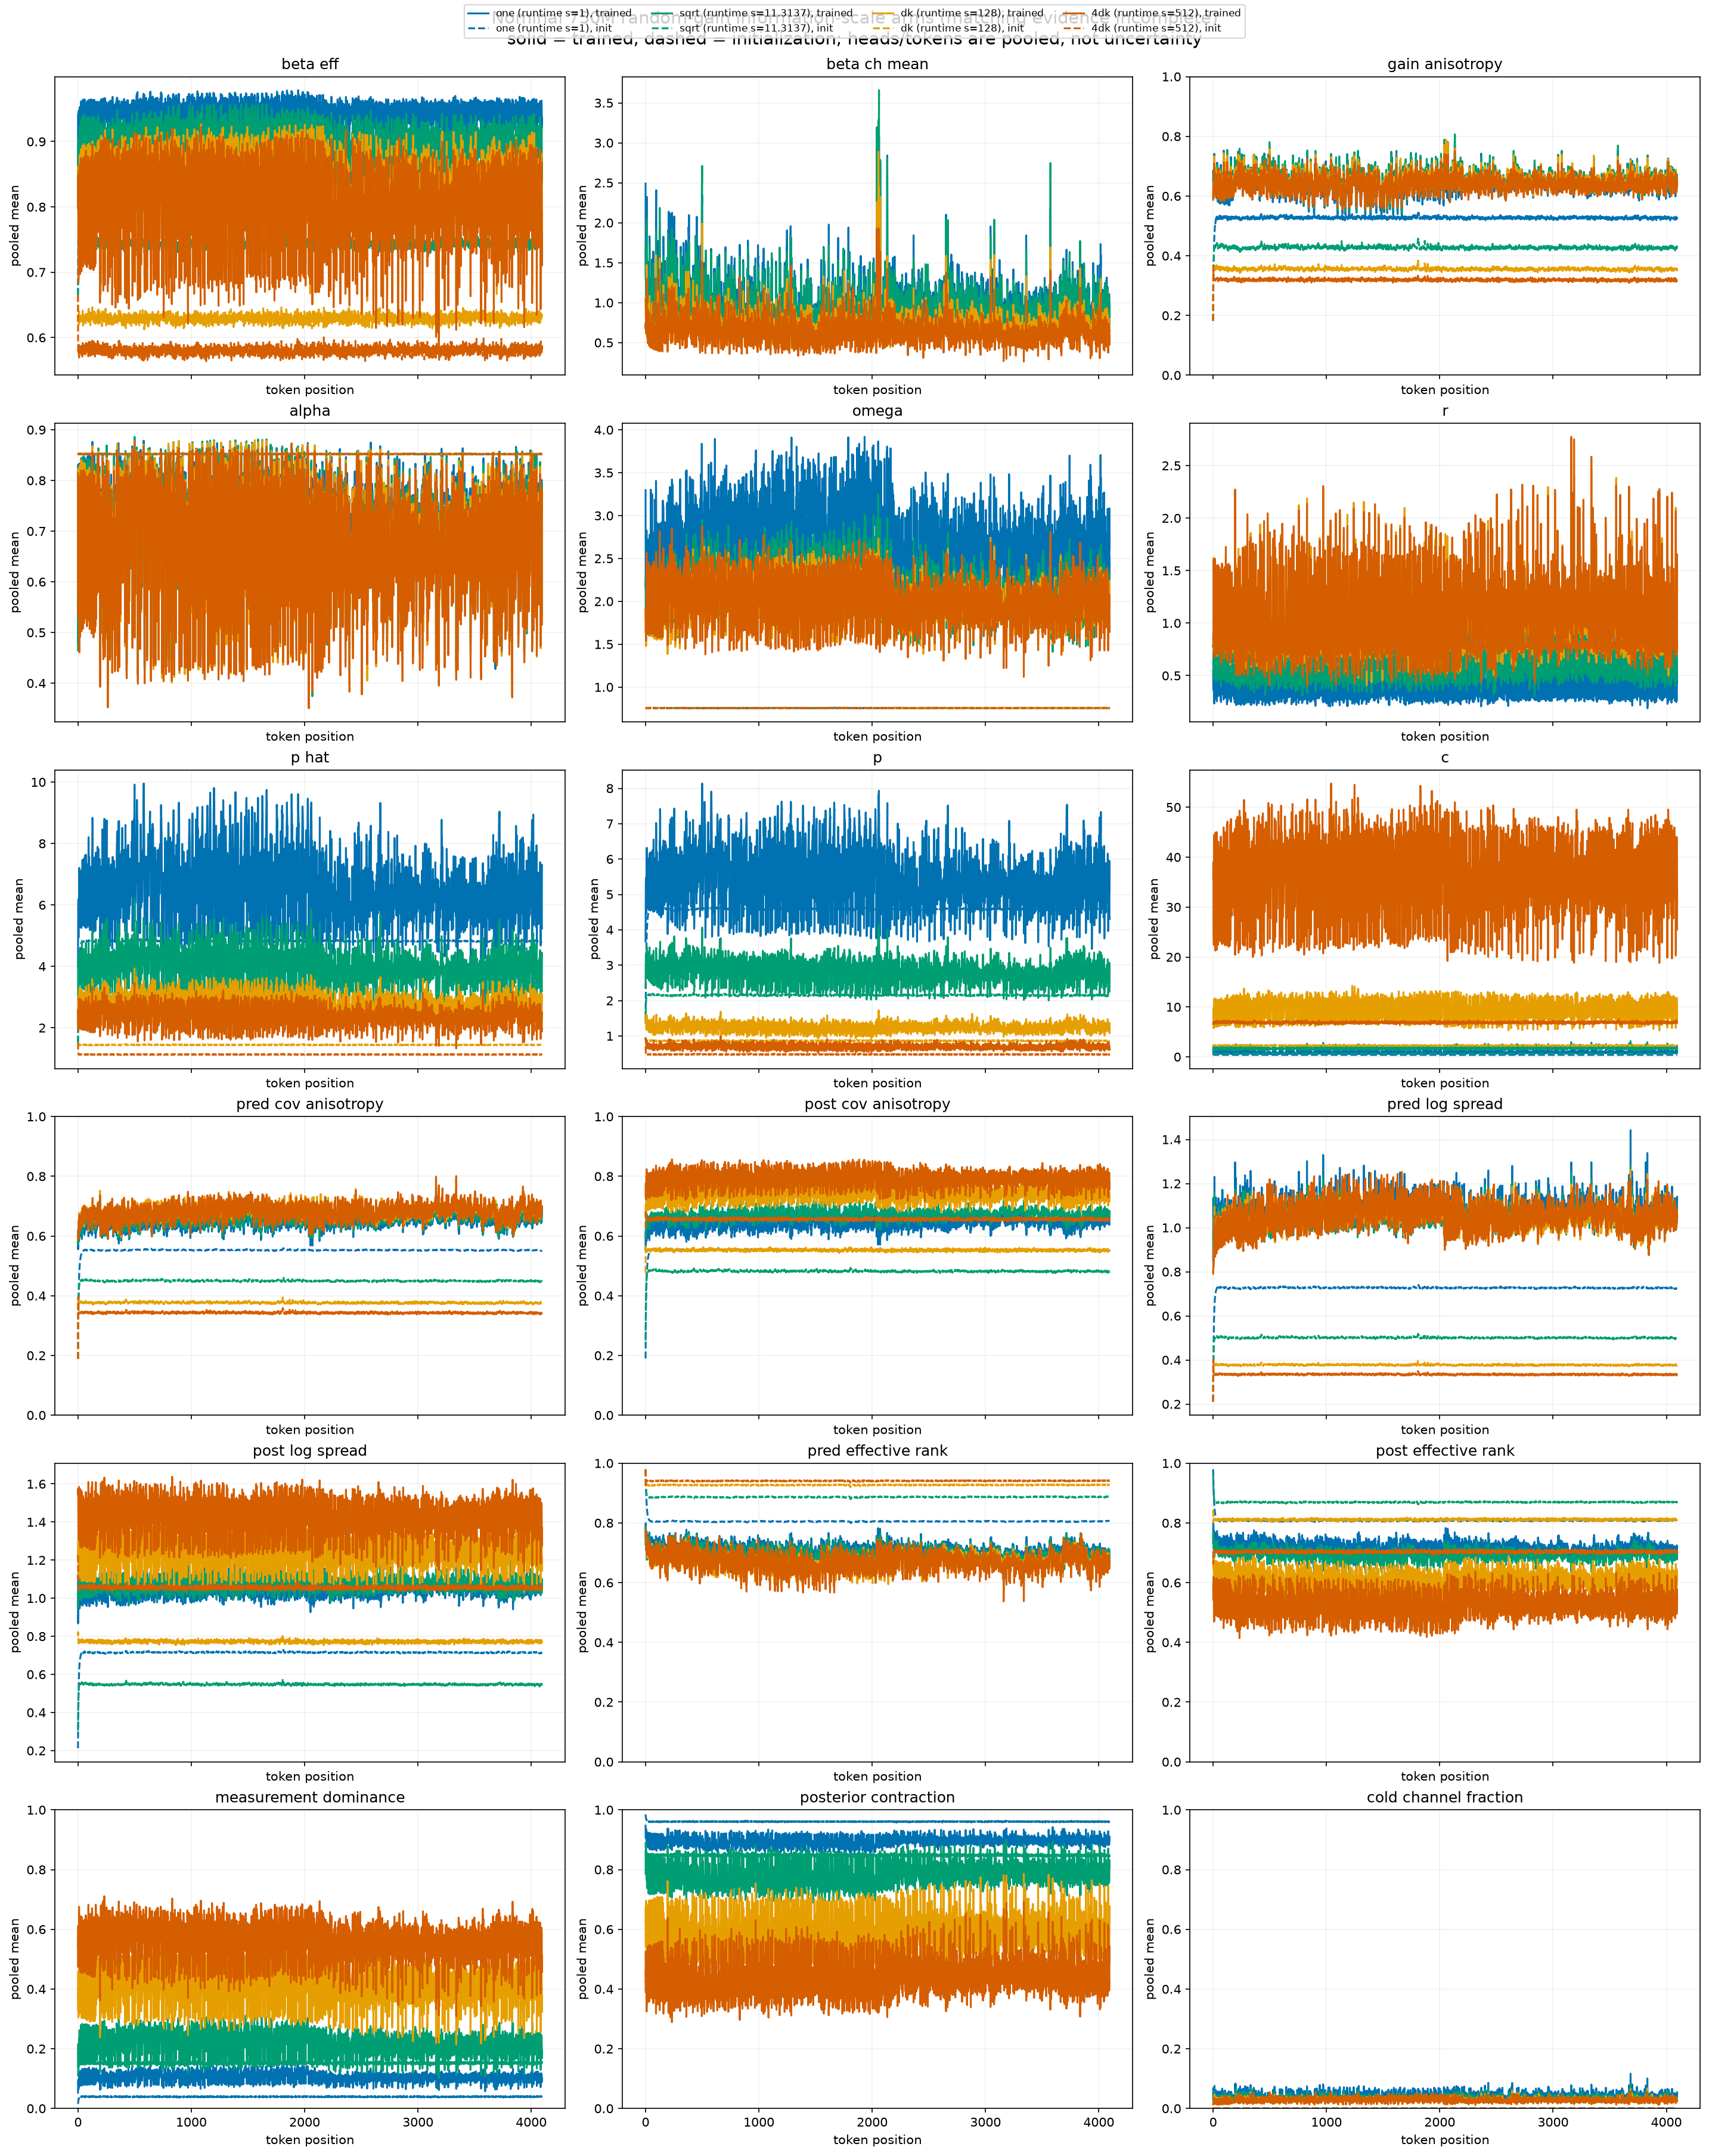
\includegraphics[height=0.84\textheight,keepaspectratio]{figures/aggregate/info_scale_trajectories.png}
\caption{Trained and canonical-initialization trajectories for the four nominal 750M
information-scale arms.  Lines summarize the same deterministic trajectory and are not
independent samples.}
\label{fig:nominal-trajectories}
\end{figure}

\begin{figure}[p]
\centering
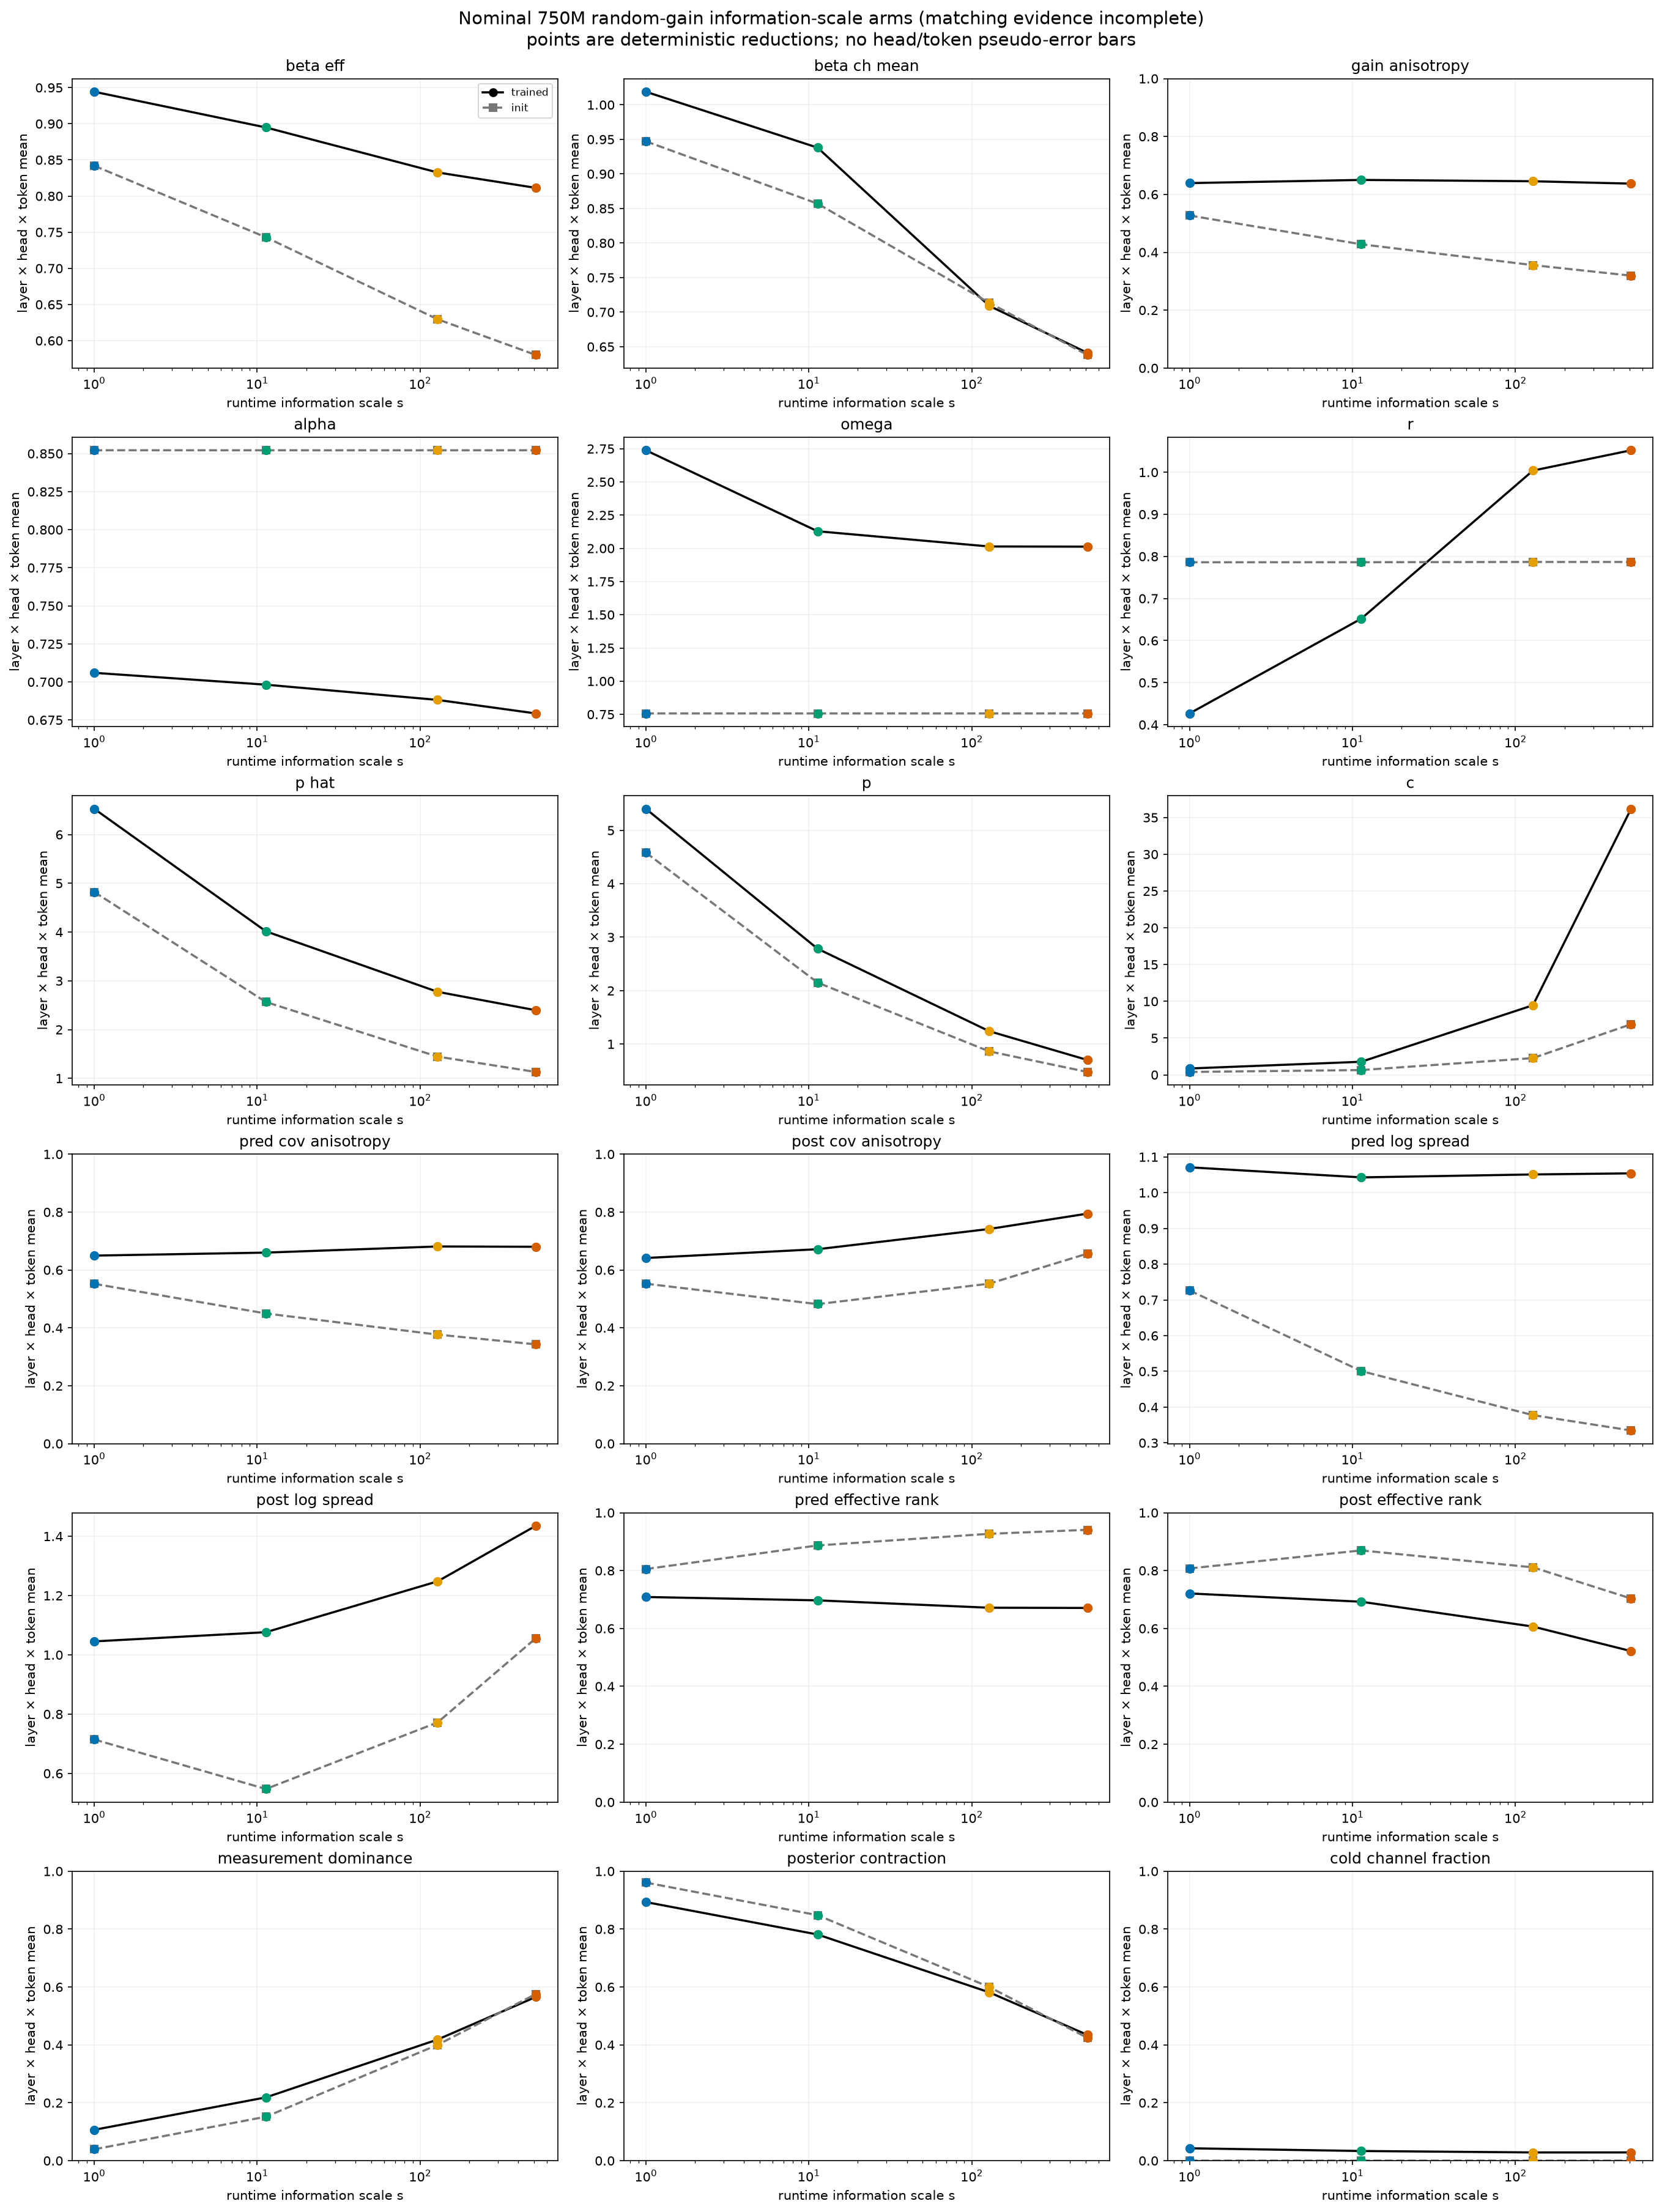
\includegraphics[height=0.84\textheight,keepaspectratio]{figures/aggregate/info_scale_variable_means.png}
\caption{Pooled internal-variable means versus nominal scale.  Connections across
checkpoints are descriptive because each point comes from independently trained weights.}
\label{fig:nominal-means}
\end{figure}

\subsection{Covariance geometry and learned anisotropy}

Table~\ref{tab:nominal-geometry} separates predicted from posterior geometry.  Predicted
anisotropy changes only modestly across $s$, from $0.650$ to about $0.680$, whereas posterior
anisotropy rises from $0.641$ to $0.795$.  The posterior-minus-predicted gap changes from
$-0.008$ at $s=1$ to $+0.114$ at $s=512$.  Thus the high-scale measurement update is an
important source of channel concentration.  Normalized posterior rank falls from $0.721$
to $0.522$ as measurement dominance rises from $0.107$ to $0.565$.

\begin{table}[htbp]
\centering
\caption{Nominal covariance geometry.  The initialization column reports gain anisotropy
from the canonical or distribution-matched control, not the historical training start.}
\label{tab:nominal-geometry}
\small
\begin{tabular}{@{}lrrrrrrrr@{}}
\toprule
$s$ & trained $\Akap$ & init $\Akap$ & $\Apre$ & $\Apost$ & $\Rpost$ & $\Mdom$ & $\Cret$ & cold \\
\midrule
$1$          & 0.639 & 0.527 & 0.650 & 0.641 & 0.721 & 0.107 & 0.893 & 0.043 \\
$\sqrt{128}$ & 0.650 & 0.428 & 0.660 & 0.672 & 0.692 & 0.219 & 0.781 & 0.033 \\
$128$        & 0.645 & 0.356 & 0.681 & 0.742 & 0.607 & 0.418 & 0.582 & 0.028 \\
$512$        & 0.637 & 0.319 & 0.680 & 0.795 & 0.522 & 0.565 & 0.435 & 0.029 \\
\bottomrule
\end{tabular}
\end{table}

Training largely erases the scale dependence of gain direction: trained $\Akap$ spans
only $0.637$--$0.650$, while the controls fall monotonically from $0.527$ to $0.319$.
Training also raises posterior anisotropy relative to its control by $0.089$, $0.190$,
$0.189$, and $0.138$ for increasing scale.  This supports learned channel selectivity,
although the controls are not exact replays of historical initialization.

\subsection{Depth dependence}

The depth profiles distinguish gain direction from covariance accumulation.  From the first
to final layer, posterior anisotropy changes $0.700\rightarrow0.737$ at $s=128$ and
$0.740\rightarrow0.788$ at $s=512$.  It is almost flat at $\sqrt{128}$ and slightly decreases
at $s=1$.  Gain anisotropy remains much flatter.  High-scale covariance concentration
therefore accumulates through recurrent state updates rather than arising solely from a
single gain projection.

\begin{table}[htbp]
\centering
\caption{First-to-last-layer trained anisotropy.}
\label{tab:depth}
\small
\begin{tabular}{@{}lccc@{}}
\toprule
$s$ & $\Akap$ & $\Apre$ & $\Apost$ \\
\midrule
$1$          & $0.663\rightarrow0.630$ & $0.676\rightarrow0.698$ & $0.680\rightarrow0.675$ \\
$\sqrt{128}$ & $0.672\rightarrow0.653$ & $0.675\rightarrow0.701$ & $0.688\rightarrow0.692$ \\
$128$        & $0.648\rightarrow0.650$ & $0.658\rightarrow0.705$ & $0.700\rightarrow0.737$ \\
$512$        & $0.642\rightarrow0.659$ & $0.652\rightarrow0.714$ & $0.740\rightarrow0.788$ \\
\bottomrule
\end{tabular}
\end{table}

\begin{figure}[p]
\centering
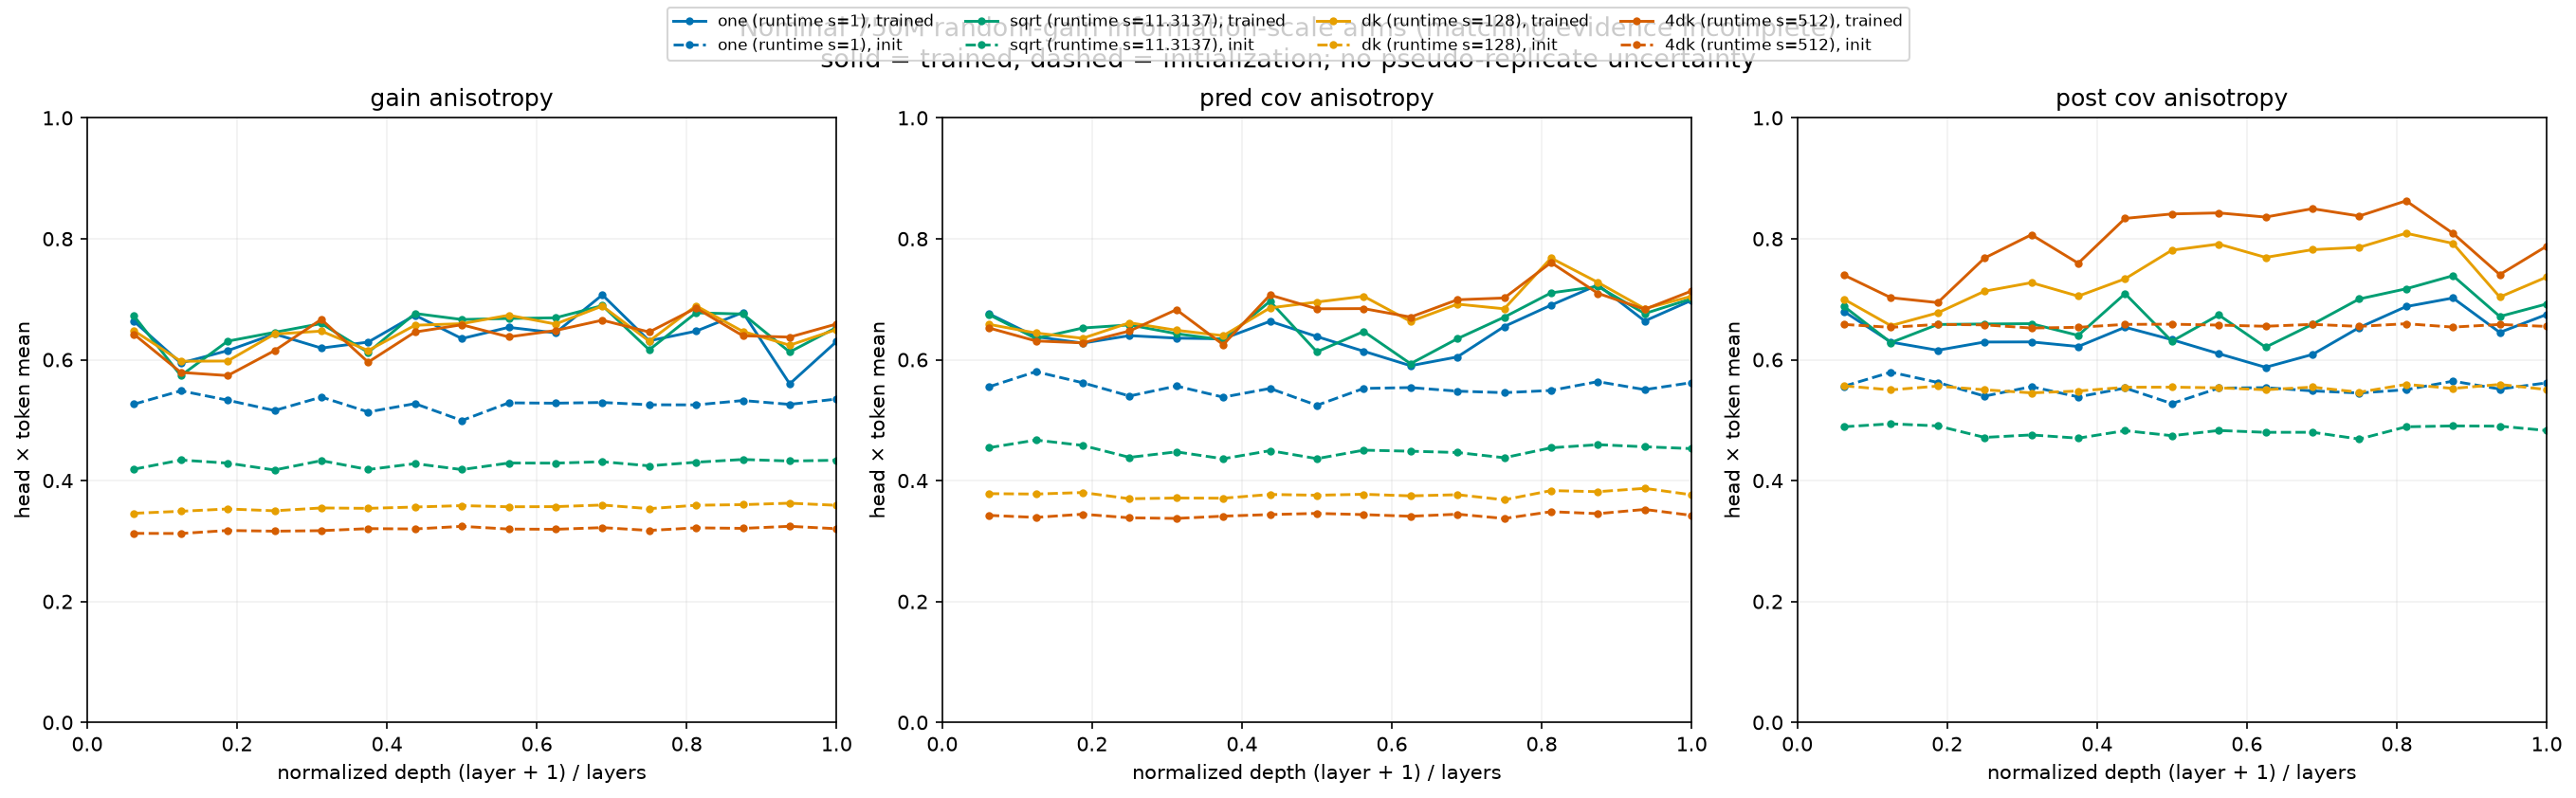
\includegraphics[width=\textwidth]{figures/aggregate/anisotropy_depth_profiles.png}
\caption{Gain and covariance anisotropy versus stored normalized depth for the four
nominal arms.}
\label{fig:depth}
\end{figure}

\section{Fixed-weight runtime-scale intervention}

The crossed grid is the strongest causal diagnostic.  Each row fixes one checkpoint trained
at $s\in\{1,\sqrt{128},128,512\}$, and each column evaluates it at one runtime scale from the
same set.  Averaged descriptively across rows, changing runtime $s$ from $1$ to $512$ raises
measurement dominance from $0.084$ to $0.559$ and reduces mean posterior covariance from
$5.585$ to $0.667$ ($88.1\%$).  Posterior anisotropy rises $0.630\rightarrow0.816$, log spread
rises $1.038\rightarrow1.475$, and normalized effective rank falls
$0.730\rightarrow0.493$.

These directions hold in every row (Table~\ref{tab:crossed-rows}).  In contrast, gain
anisotropy rises only $0.025$--$0.036$, while mean channel gain falls by
$0.369$--$0.591$.  Runtime scale therefore has a strong effect on covariance magnitude and
channel concentration, but only a modest effect on the angle of the gain relative to the key.

\begin{table}[htbp]
\centering
\caption{Endpoint changes for fixed weights, runtime $s:1\rightarrow512$.  The $p$ column
is percent change; all other columns are absolute changes.}
\label{tab:crossed-rows}
\resizebox{\textwidth}{!}{%
\begin{tabular}{@{}lrrrrrrr@{}}
\toprule
Training $s$ & $\Delta\Mdom$ & $\Delta p$ & $\Delta\Apost$ &
$\Delta\operatorname{std}(\log p)$ & $\Delta\Rpost$ & $\Delta\Akap$ &
$\Delta\overline\beta_{\rm ch}$ \\
\midrule
$1$          & +0.489 & $-88.9\%$ & +0.212 & +0.509 & $-0.289$ & +0.036 & $-0.369$ \\
$\sqrt{128}$ & +0.467 & $-88.3\%$ & +0.193 & +0.438 & $-0.242$ & +0.036 & $-0.558$ \\
$128$        & +0.469 & $-87.8\%$ & +0.176 & +0.398 & $-0.215$ & +0.036 & $-0.576$ \\
$512$        & +0.476 & $-87.3\%$ & +0.166 & +0.401 & $-0.204$ & +0.025 & $-0.591$ \\
\bottomrule
\end{tabular}}
\end{table}

Table~\ref{tab:crossed-all} records the mean endpoint change for every trajectory variable.
The nearly unchanged $\alpha$, $\omega$, and $r$ should not be read as a direct algebraic
invariance: intervening at every layer changes the downstream inputs from which those values
are predicted.  Their small changes instead show that the dominant response lies in the
information/covariance recursion.  The exact equality
$\Delta\Cret=-\Delta\Mdom$ is a useful consistency check.

\begin{table}[htbp]
\centering
\caption{Across-row mean endpoints for every crossed-grid trajectory variable.}
\label{tab:crossed-all}
\small
\begin{tabular}{@{}lrrr@{}lrrr@{}}
\toprule
Variable & $s=1$ & $s=512$ & $\Delta$ & Variable & $s=1$ & $s=512$ & $\Delta$ \\
\midrule
$\beta_{\rm eff}$ & 0.886 & 0.857 & $-0.030$ & $\Apre$ & 0.629 & 0.720 & +0.091 \\
$\overline\beta_{\rm ch}$ & 1.166 & 0.643 & $-0.523$ & $\Apost$ & 0.630 & 0.816 & +0.187 \\
$\Akap$ & 0.622 & 0.655 & +0.033 & pred. log spread & 1.037 & 1.167 & +0.131 \\
$\bar\alpha$ & 0.676 & 0.679 & +0.003 & post. log spread & 1.038 & 1.475 & +0.437 \\
$\bar\omega$ & 2.136 & 2.047 & $-0.089$ & pred. eff. rank & 0.729 & 0.616 & $-0.113$ \\
$r$ & 0.790 & 0.803 & +0.013 & $\Rpost$ & 0.730 & 0.493 & $-0.237$ \\
$\overline{\widehat p}$ & 6.363 & 2.430 & $-3.933$ & $\Mdom$ & 0.084 & 0.559 & +0.475 \\
$\bar p$ & 5.585 & 0.667 & $-4.918$ & $\Cret$ & 0.916 & 0.441 & $-0.475$ \\
$\bar c$ & 0.936 & 38.263 & +37.328 & cold fraction & 0.043 & 0.037 & $-0.006$ \\
\bottomrule
\end{tabular}
\end{table}

\begin{figure}[p]
\centering
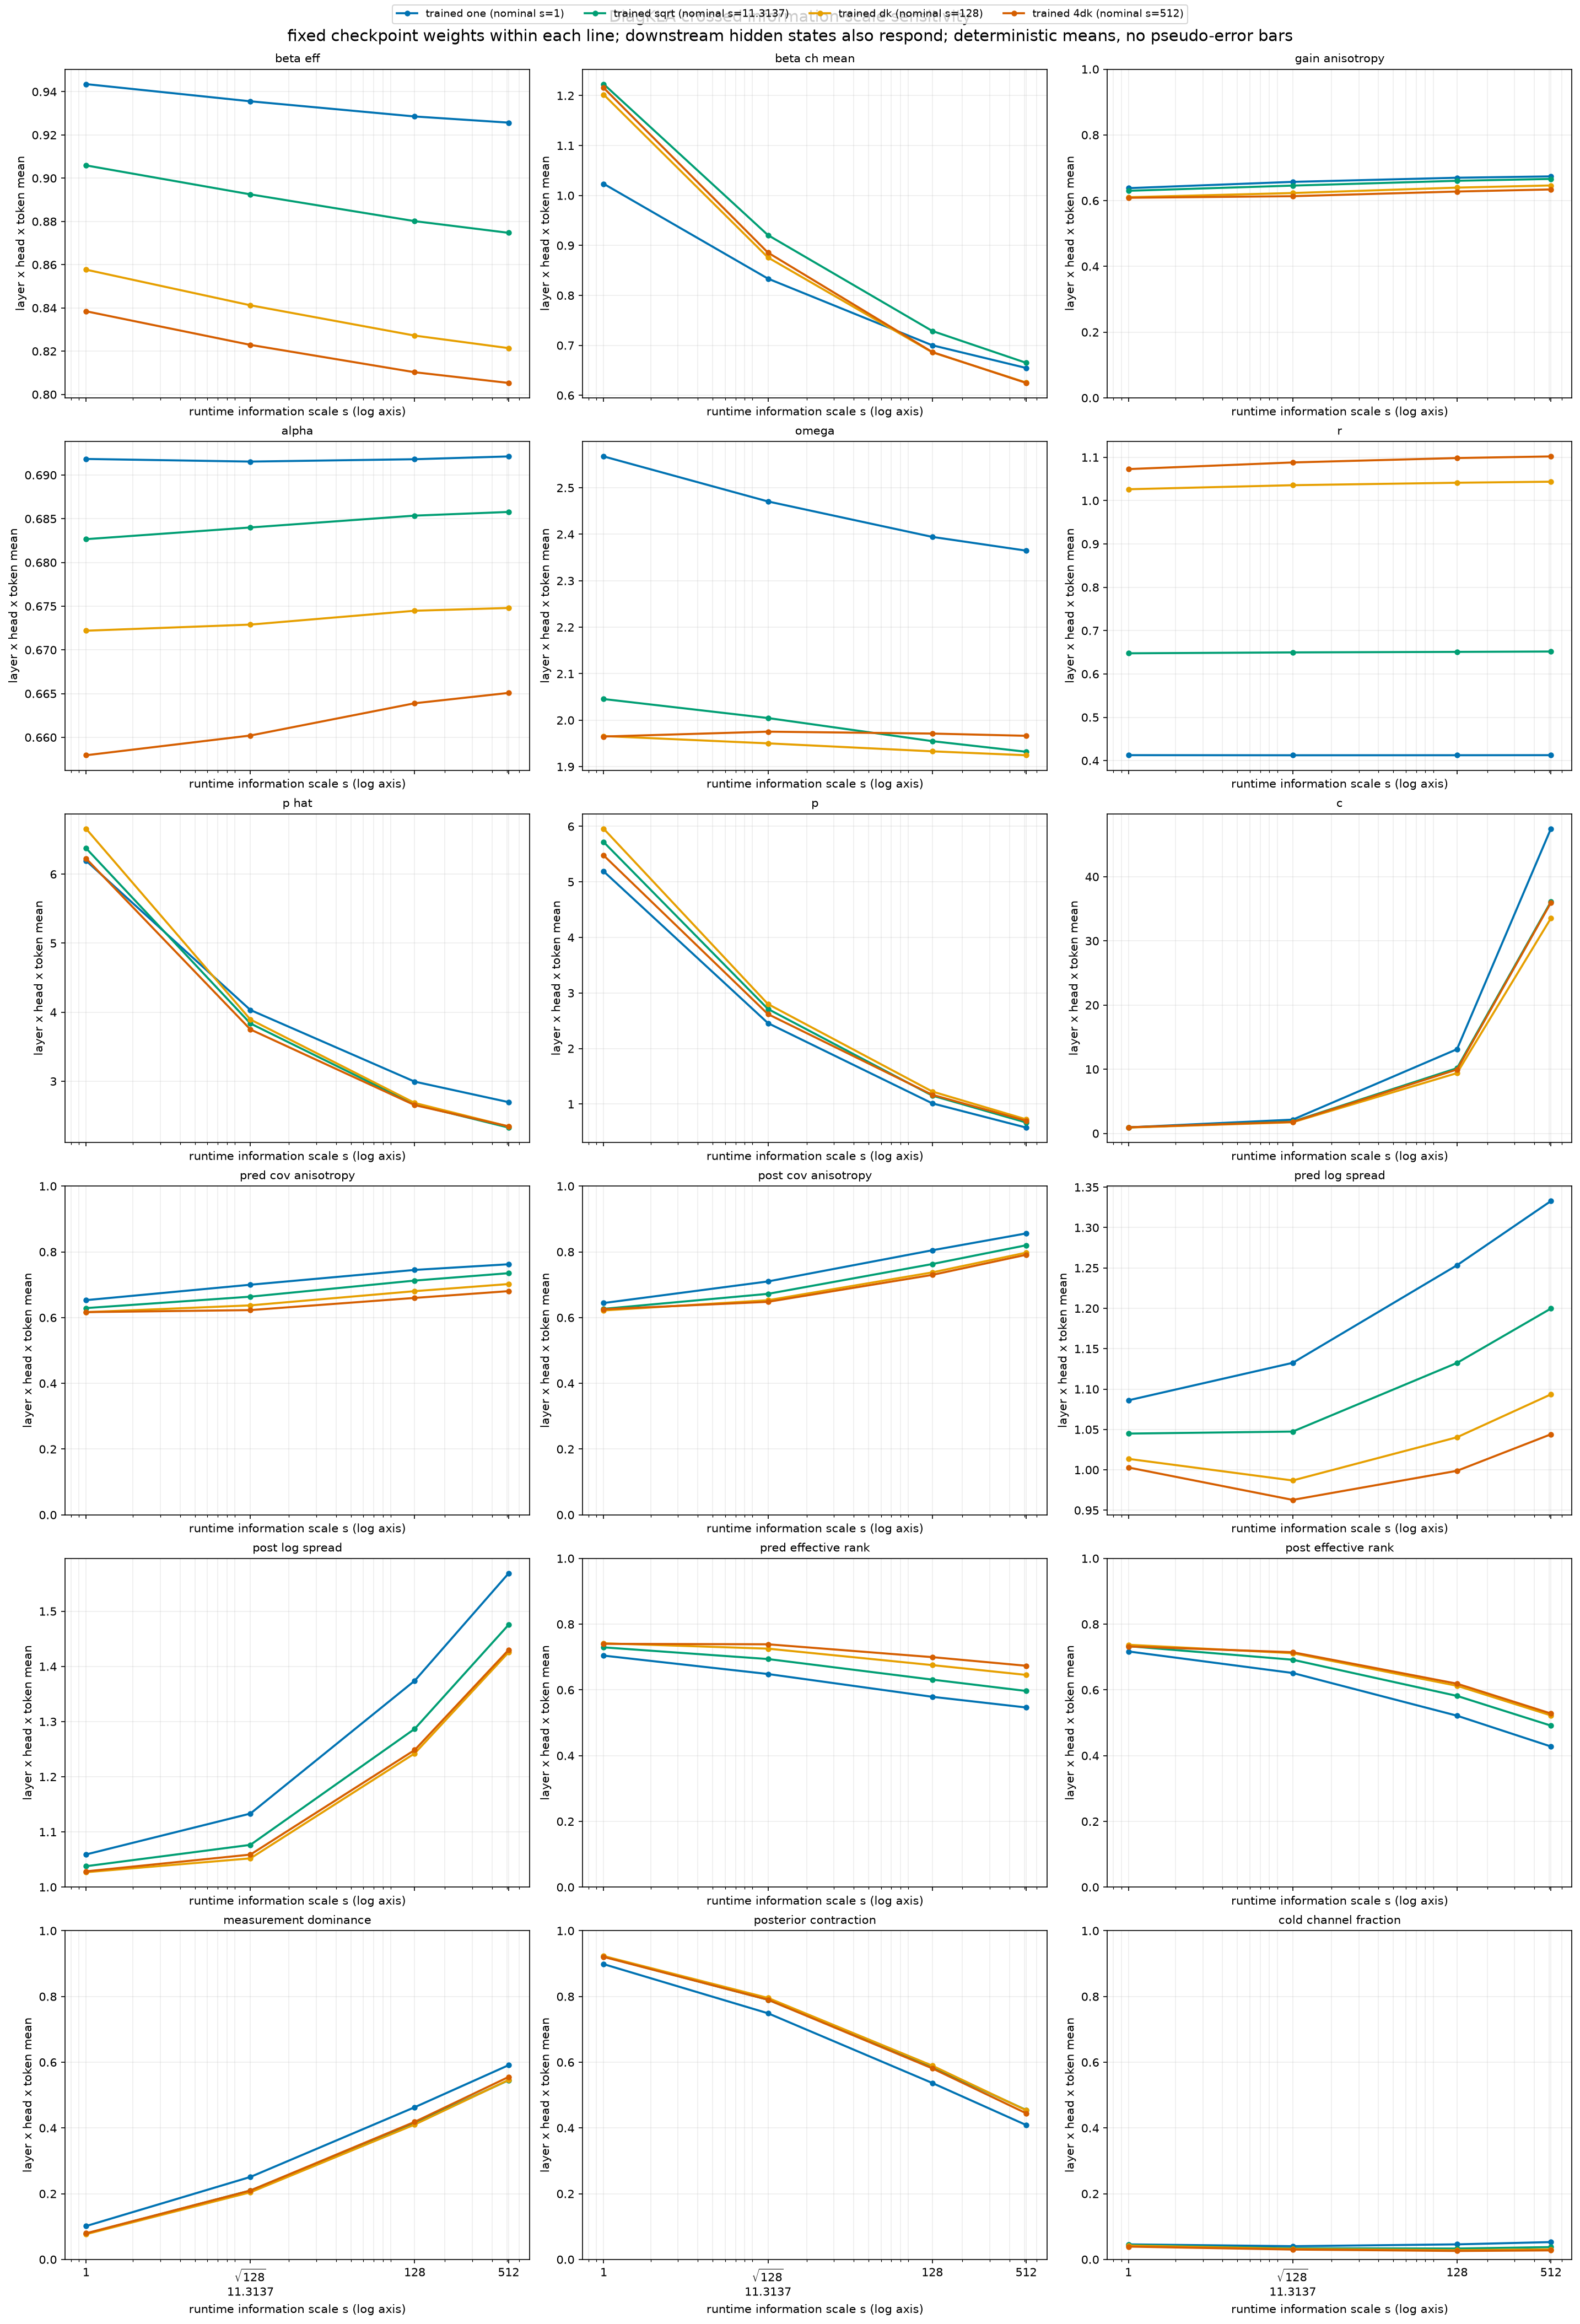
\includegraphics[height=0.85\textheight,keepaspectratio]{figures/aggregate/crossed_info_scale_sensitivity.png}
\caption{All trajectory variables versus runtime scale.  Each line fixes one trained
checkpoint; the intervention acts at every layer.}
\label{fig:crossed-sensitivity}
\end{figure}

\begin{figure}[p]
\centering
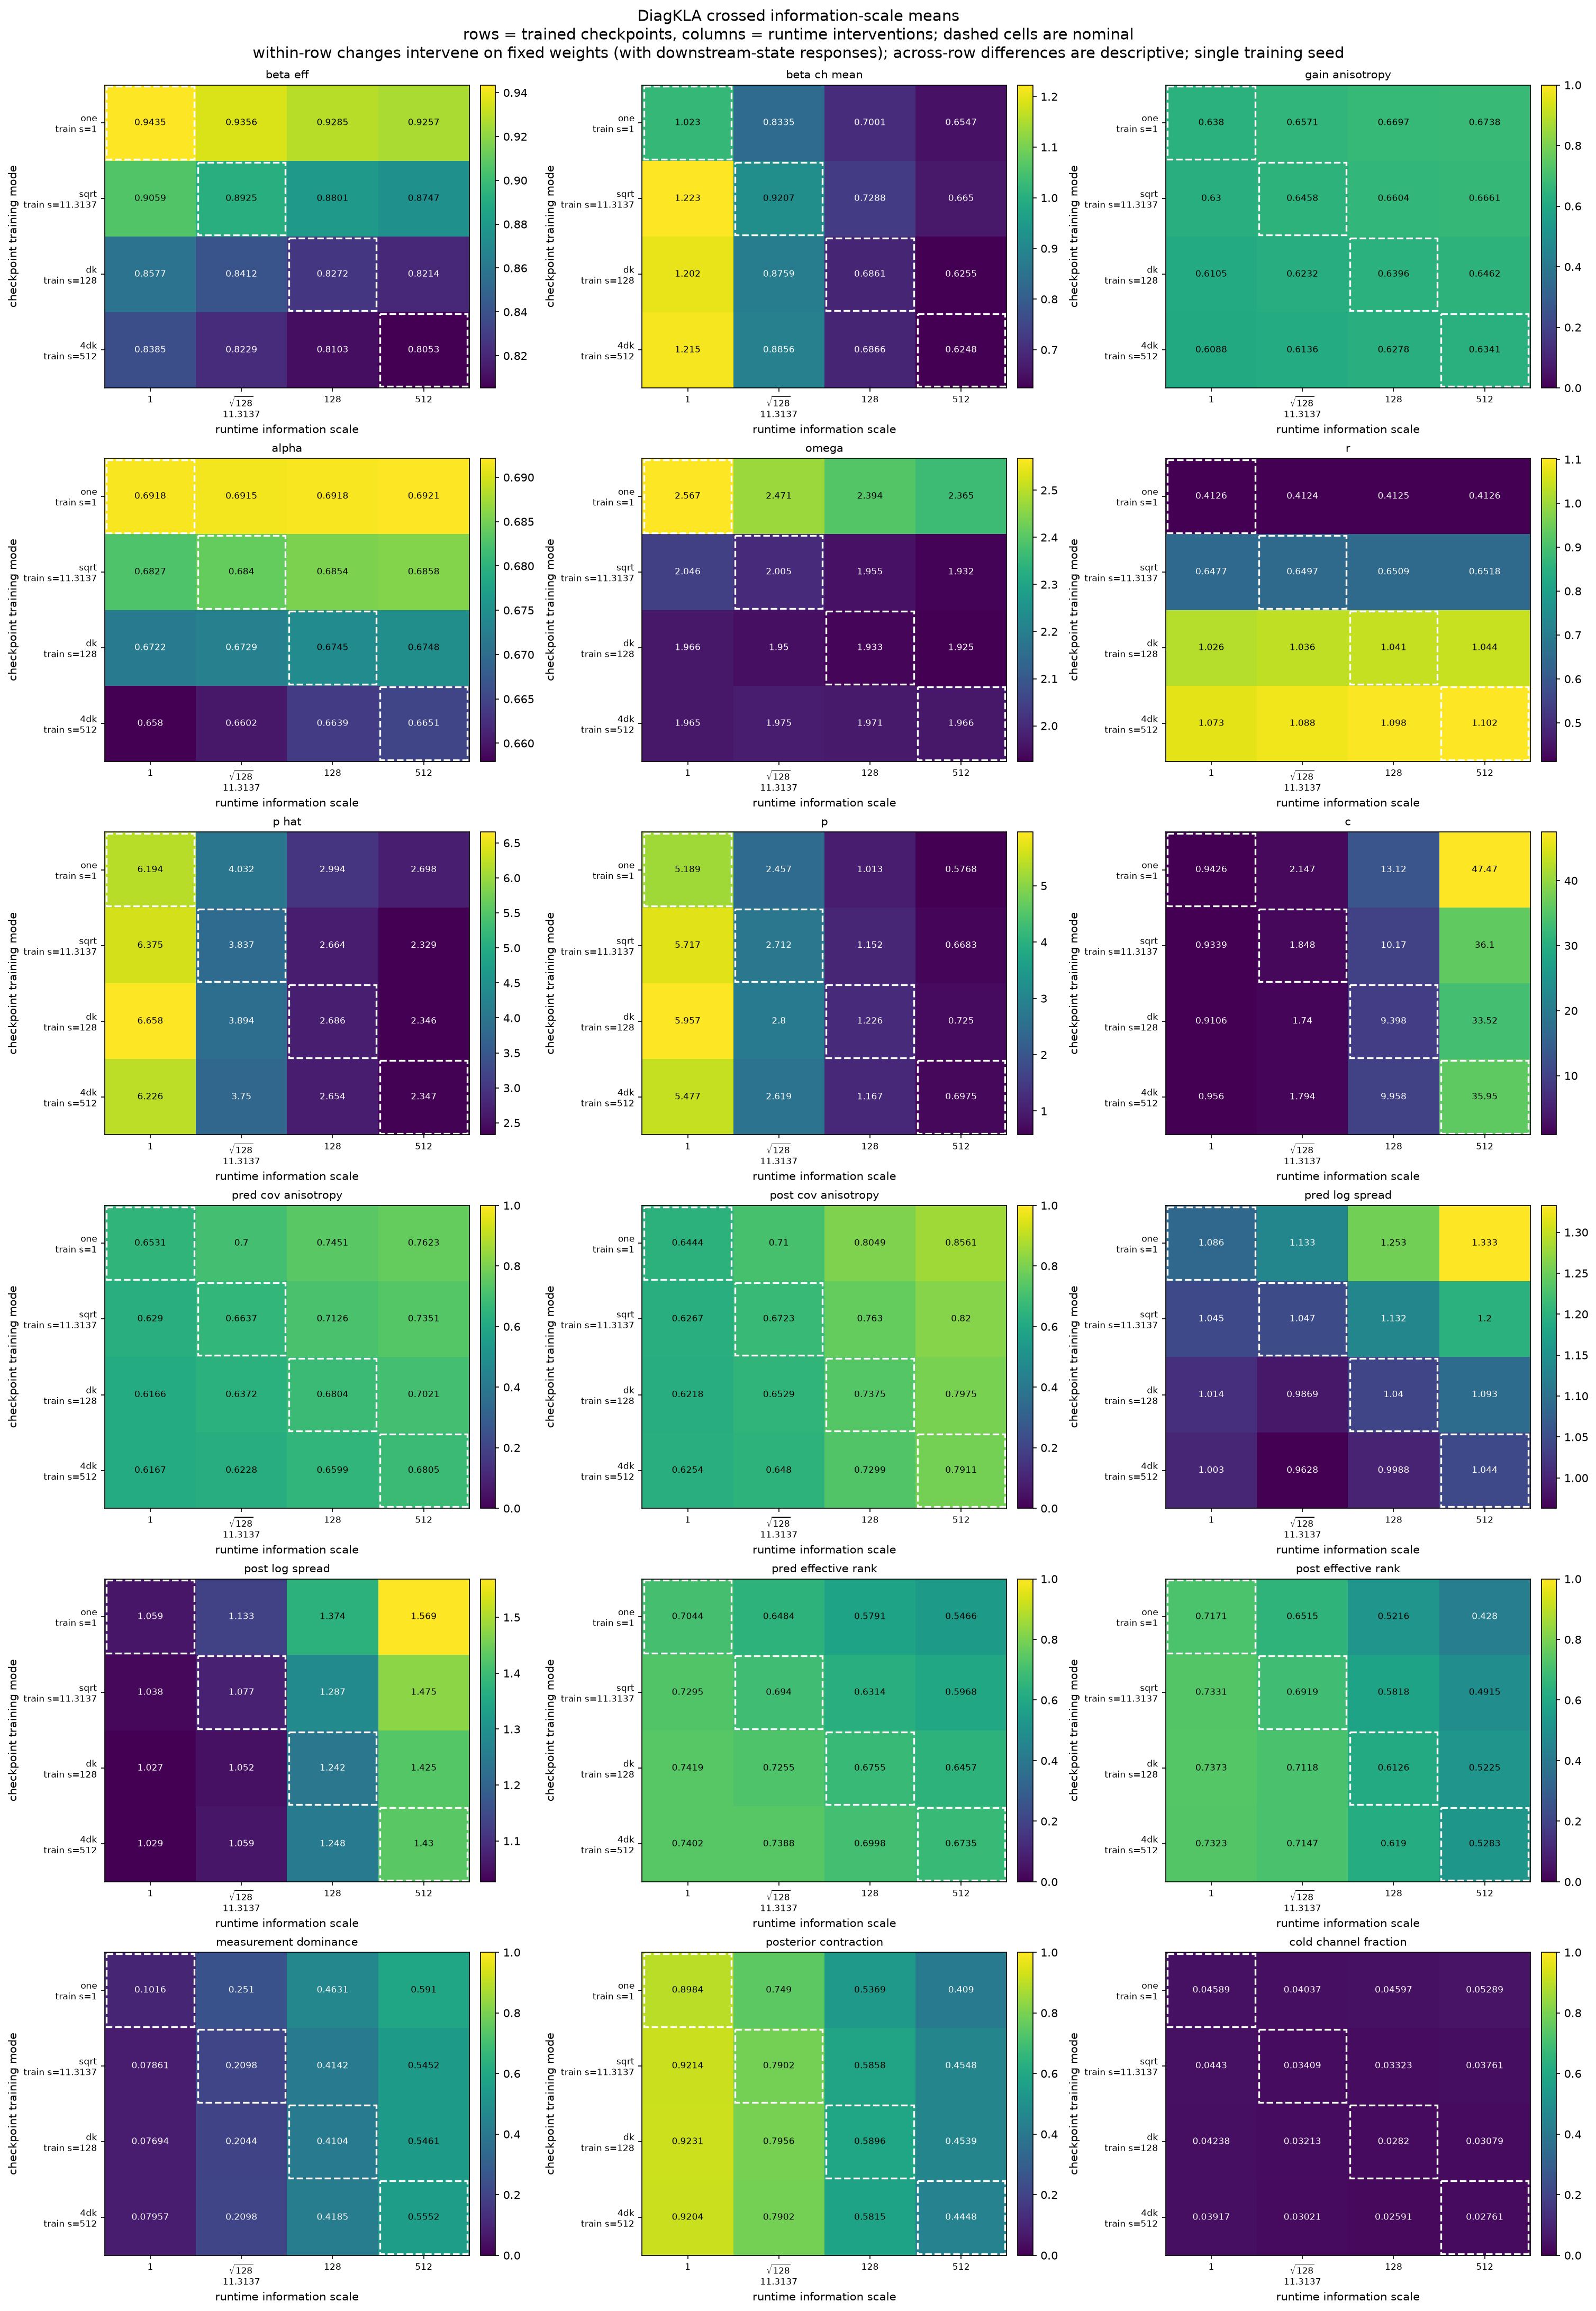
\includegraphics[height=0.85\textheight,keepaspectratio]{figures/aggregate/crossed_info_scale_heatmaps.png}
\caption{Crossed pooled means.  Rows are training scales, columns are runtime scales, and
dashed cells mark nominal train/runtime matches.}
\label{fig:crossed-heatmaps}
\end{figure}

\section{Initialization, implementation, and model-size controls}

\paragraph{Initialization and available seed control.}
At nominal $s=128$, current random-gain R11 and isotropic-init R07--R08 are close after 50B
tokens.  Their gain anisotropy is $0.645$--$0.651$, posterior anisotropy is
$0.742$--$0.757$, and measurement dominance is $0.418$--$0.432$.  The two isotropic-init
runs differ by only $0.005$ in posterior anisotropy.  This is descriptive robustness across
two available controls, not a seed study: one seed is unrecorded and there are no replicate
random-gain seeds.

\paragraph{Historical-code controls.}
The three old-code checkpoints cluster even more tightly: gain anisotropy
$0.650$--$0.651$, posterior anisotropy $0.756$--$0.758$, normalized posterior rank
$0.583$--$0.586$, and measurement dominance $0.430$--$0.434$.  Strict loading verifies
tensor/schema compatibility with the current probe but cannot establish that historical
training code had identical runtime semantics.

\paragraph{Model size and budget.}
R02 (220M/20B), R11 (750M/50B), and R01 (1.3B/100B) have nearly constant gain anisotropy
($0.643$, $0.645$, $0.646$), while posterior anisotropy increases
$0.707\rightarrow0.742\rightarrow0.753$ and measurement dominance increases
$0.327\rightarrow0.418\rightarrow0.477$.  Head dimension, nominal numerical scale, model
size, and training tokens all change together, so this is not an identified size effect.

\section{Mechanistic interpretation}

Three observations fit one coherent picture.
\begin{enumerate}
  \item \textbf{Training learns directional selectivity.}  Trained gain anisotropy converges
  near $0.64$ across the four nominal scales, far above the high-scale initialization
  controls.  The gain is therefore not well summarized as a scalar multiple of the key.
  \item \textbf{Scale controls uncertainty concentration more than gain angle.}  At fixed
  weights, increasing $s$ adds channel-wise measurement information proportional to $k_i^2$.
  The posterior becomes smaller, more unequal across channels, and lower rank.  Mean gain
  falls strongly, while its off-key fraction changes only slightly.
  \item \textbf{High-scale concentration accumulates with depth.}  The deeper layers of the
  $s=128$ and $s=512$ checkpoints show increasing posterior anisotropy, whereas low-scale
  profiles are nearly flat.  The covariance state carries channel-specific evidence across
  tokens and layers rather than merely reflecting one instantaneous key.
\end{enumerate}

The low cold-channel fraction matters for interpretation.  A high anisotropy score could be
produced by broadly collapsing most channels to zero, but only $2.6\%$--$5.3\%$ of crossed
cells' channels satisfy the cold threshold.  The observed reduction in effective rank is
therefore distributed channel concentration under this diagnostic, not wholesale channel
death.

\section{Limitations and reading guide}

\begin{itemize}
  \item There is one checkpoint per training arm.  Heads, layers, and tokens are dependent
  measurements, not seed replicates; no pseudo-error bars or population claims are made.
  \item Nominal arms are not proven byte-identical in seed, data order, and historical code.
  Across-row comparisons are descriptive.
  \item Initialization artifacts are canonical or distribution-matched controls generated
  with analysis seed 0.  They are not exact historical initialization replays.
  \item All results describe deterministic token sequences, not an estimate over the
  FineWeb-Edu population.
  \item Runtime interventions are causal within a row but act on the complete multilayer
  network, not on one isolated recurrence.
  \item Current-code strict loading and source hashes do not prove historical-code
  equivalence for the old checkpoints.
  \item Gain histograms share a display window.  Trained
  $\beta_{\mathrm{ch}}$ has 16,151, 14,954, 6,504, and 4,286 upper-tail samples outside that
  window for $s=1,\sqrt{128},128,512$; the numeric trajectory reductions remain untrimmed.
  \item No downstream evaluation is performed after removing or equalizing anisotropy.
  A causal performance test would isotropize $\widehat p$ or $p$ while preserving a chosen
  scalar statistic and then measure loss/retrieval under the same token stream.
\end{itemize}

\section{Conclusion}

DiagKLA checkpoints learn strongly channel-dependent covariance and gain.  The stable trained
gain anisotropy near $0.64$ shows that this behavior persists across a 512-fold nominal scale
range after training.  Information scale nevertheless remains a powerful state-control
parameter: at fixed weights it transfers the update from prior retention toward measurement
information, shrinks posterior covariance by about $88\%$, raises posterior anisotropy by
$0.17$--$0.21$, and lowers normalized effective rank by $0.20$--$0.29$.  The dominant scale
effect is therefore covariance contraction and channel concentration, not a large rotation of
the gain.  These findings motivate a trace-preserving isotropization ablation if the next goal
is to connect learned anisotropy causally to language-model performance.

\appendix
\section{All-checkpoint trained summary}

Table~\ref{tab:all-runs} reports the same deterministic pooled metrics for all eleven
checkpoints.  The full trained and initialization-control figures follow in
Appendix~\ref{app:checkpoint-pages}.

\begin{table}[htbp]
\centering
\caption{All-checkpoint trained trajectory means.}
\label{tab:all-runs}
\resizebox{\textwidth}{!}{%
\begin{tabular}{@{}llllrrrrrr@{}}
\toprule
Alias & Model & Family & $s$ & $\Akap$ & $\Apre$ & $\Apost$ & $\Rpost$ & $\Mdom$ & cold \\
\midrule
R01 & 1.3B & random & 128 & 0.646 & 0.675 & 0.753 & 0.591 & 0.477 & 0.026 \\
R02 & 220M & random & 64 & 0.643 & 0.682 & 0.707 & 0.649 & 0.327 & 0.020 \\
R03 & 750M & old B200 & 128 & 0.651 & 0.691 & 0.756 & 0.586 & 0.430 & 0.039 \\
R04 & 750M & old GDN2-mem & 128 & 0.650 & 0.690 & 0.758 & 0.583 & 0.434 & 0.038 \\
R05 & 750M & old H100 & 128 & 0.650 & 0.692 & 0.758 & 0.583 & 0.433 & 0.037 \\
R06 & 750M & random & 512 & 0.637 & 0.680 & 0.795 & 0.522 & 0.565 & 0.029 \\
R07 & 750M & isotropic-init & 128 & 0.651 & 0.691 & 0.757 & 0.585 & 0.432 & 0.038 \\
R08 & 750M & isotropic-init s1234 & 128 & 0.650 & 0.687 & 0.753 & 0.590 & 0.425 & 0.035 \\
R09 & 750M & random & 1 & 0.639 & 0.650 & 0.641 & 0.721 & 0.107 & 0.043 \\
R10 & 750M & random & $\sqrt{128}$ & 0.650 & 0.660 & 0.672 & 0.692 & 0.219 & 0.033 \\
R11 & 750M & random & 128 & 0.645 & 0.681 & 0.742 & 0.607 & 0.418 & 0.028 \\
\bottomrule
\end{tabular}}
\end{table}

\clearpage
\section{Per-checkpoint diagnostics}
\label{app:checkpoint-pages}

Each page contains all six plots for one checkpoint.  The left column is the trained
checkpoint; the right column is its canonical or distribution-matched initialization
control.  These controls use the current model construction and analysis seed and should not
be mistaken for saved historical initial states.

\RunDiagnostics{R01}{tsz128x4k_100B_diag_kla_1.3B_randgain_repro_ngocbh_diag_kla_1.3B_100B_randgain}{1.3B random-gain, 100B tokens}{Nominal $s=128$; $\Akap=0.646$, $\Apost=0.753$, $\Rpost=0.591$, $\Mdom=0.477$.}

\RunDiagnostics{R02}{tsz128x4k_20B_repro_ngocbh_diag_kla_220M_randgain_20B}{220M random-gain, 20B tokens}{Head dimension 64 and nominal $s=64$; $\Akap=0.643$, $\Apost=0.707$, $\Rpost=0.649$, $\Mdom=0.327$.}

\RunDiagnostics{R03}{tsz128x4k_50B_repro_ngocbh_diag_kla_750M_50B_isdk_oldcode_b200_v2}{750M old-code B200 v2}{Nominal $s=128$; historical gain initialization unknown; $\Apost=0.756$, $\Mdom=0.430$.}

\RunDiagnostics{R04}{tsz128x4k_50B_repro_ngocbh_diag_kla_750M_50B_isdk_oldcode_gdn2mem_h100}{750M old-code GDN2-memory H100}{Nominal $s=128$; historical gain initialization unknown; $\Apost=0.758$, $\Mdom=0.434$.}

\RunDiagnostics{R05}{tsz128x4k_50B_repro_ngocbh_diag_kla_750M_50B_isdk_oldcode_h100}{750M old-code H100}{Nominal $s=128$; historical gain initialization unknown; $\Apost=0.758$, $\Mdom=0.433$.}

\RunDiagnostics{R06}{tsz128x4k_50B_repro_ngocbh_diag_kla_750M_is4dk_randgain_50B}{750M random-gain, $s=512$}{Highest nominal scale; $\Akap=0.637$, $\Apost=0.795$, $\Rpost=0.522$, $\Mdom=0.565$.}

\RunDiagnostics{R07}{tsz128x4k_50B_repro_ngocbh_diag_kla_750M_isdk_isoinit_50B}{750M isotropic-init}{Nominal $s=128$, seed unrecorded; $\Akap=0.651$, $\Apost=0.757$, $\Mdom=0.432$.}

\RunDiagnostics{R08}{tsz128x4k_50B_repro_ngocbh_diag_kla_750M_isdk_isoinit_s1234_50B}{750M isotropic-init, seed 1234}{Nominal $s=128$; $\Akap=0.650$, $\Apost=0.753$, $\Mdom=0.425$.}

\RunDiagnostics{R09}{tsz128x4k_50B_repro_ngocbh_diag_kla_750M_isone_randgain_50B}{750M random-gain, $s=1$}{Lowest nominal scale; $\Akap=0.639$, $\Apost=0.641$, $\Rpost=0.721$, $\Mdom=0.107$.}

\RunDiagnostics{R10}{tsz128x4k_50B_repro_ngocbh_diag_kla_750M_issqrt_randgain_50B}{750M random-gain, $s=\sqrt{128}$}{Nominal $s\approx11.314$; $\Akap=0.650$, $\Apost=0.672$, $\Rpost=0.692$, $\Mdom=0.219$.}

\RunDiagnostics{R11}{tsz128x4k_50B_repro_ngocbh_diag_kla_750M_randgain_50B}{750M random-gain, $s=128$}{Current central arm; $\Akap=0.645$, $\Apost=0.742$, $\Rpost=0.607$, $\Mdom=0.418$.}

\end{document}
